% !TEX root=../main.tex

\section{Introduction}\label{sec:intro}

During aggressive maneuvers, vision-based perception techniques tend to fail because of the lack of tracked features.
This is a well-known issue and is commonly reported in the literature (see for example,~\cite{Shen2013,Falanga2017}).
The purpose of this project is to mitigate loss of feature tracks by being more clever in which features to use for graph-based state estimation.
This adds robustness to the visual-inertial motion estimation pipeline by disregarding features that are predicted to soon be lost based on future robot motion.
Further, we allow for more efficient optimization by using fewer features with high information content.

This project accomplishes these goals by incorporating the attention and anticipation formulation of Carlone~\cite{Carlone2017} with the fixed-lag smoother of VINS-Mono~\cite{Qin2018}, a recent state-of-the-art implementation of visual-inertial odometry.
The resulting implementation is publicly available\footnote{\url{https://github.com/plusk01/Anticipated-VINS-Mono}} and is referred to as \texttt{Anticipated VINS-Mono}.
A high-level system architecture diagram is shown in Figure~\ref{fig:architecture}.

Related to the goal of robust vision-based state estimation during flight is the idea of active vision.
An early example of being selective with which features to select was provided by Davison~\cite{Davison2005}.
In his work, multual information is used to extract priors that inform feature tracking algorithms on where to look.
Yu and Beard~\cite{Yu2013} formulate a vision-based collision avoidance technique for MAVs that simultaneously minimizes state estimation uncertainties while avoiding obstacle collisions.
Falanga et al.~\cite{Falanga2018} presented a model predictive control (MPC) framework that unifies both control and perception objectives---allowing a multirotor to optimally fulfill its mission and maximize visibility of a point of interest.
The ideas of active vision can be summarized by psychologist Eleanor J. Gibson on the human learning behaviors: ``we don't simply see, we look''~\cite{Gibson1988}.

\begin{figure}
\centering
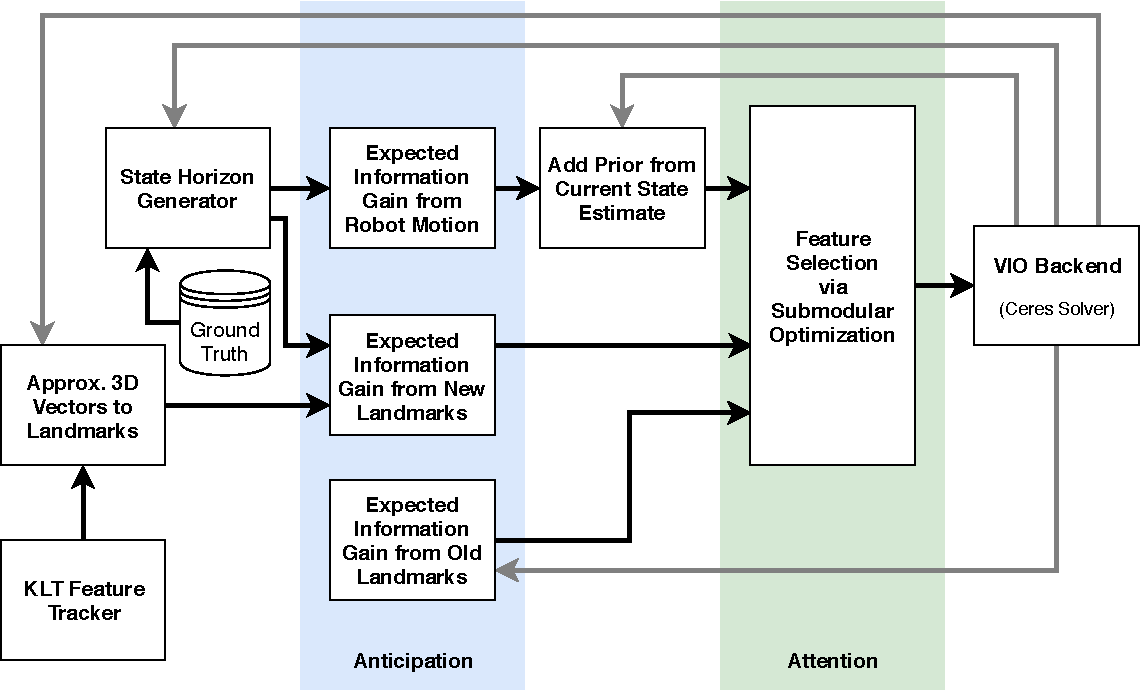
\includegraphics[width=\columnwidth]{architecture.pdf} 
\caption{System architecture of \texttt{Anticipated VINS-Mono}. All blocks are new except for the VIO back end, the core VINS-Mono component.}
\label{fig:architecture} 
\end{figure}

The rest of this paper is organized as follows.
In Section~\ref{sec:vinsmono} we discuss concepts related to visual-inertial odometry and an overview of VINS-Mono.
In Section~\ref{sec:anticipation} we provide details of our implementation of attention and anticipation.
In Section~\ref{sec:results} we give results.
Finally, we conclude in Section~\ref{sec:conclusion}.
